When using the \openshmem \ac{API}, synchronization, ordering, and completion of
communication become critical. The updates via \PUT{} routines, \acp{AMO}, stores, and
nonblocking \PUT{} and \GET{} routines on symmetric data cannot be guaranteed until some form of
synchronization or ordering is introduced in the user's program. The table below
gives the different synchronization and ordering choices, and the situations
where they may be useful.\\

\begin{tabular}{p{0.2\textwidth} | p{0.7\textwidth}}
\hline
\textbf{\openshmem  \ac{API}} & \centering \textbf{Working of \openshmem \ac{API}} \tabularnewline
\hline
\hline
{Point-to-point synchronization}\\
\FUNC{shmem\_wait\_until}
&
\raisebox{-\totalheight}{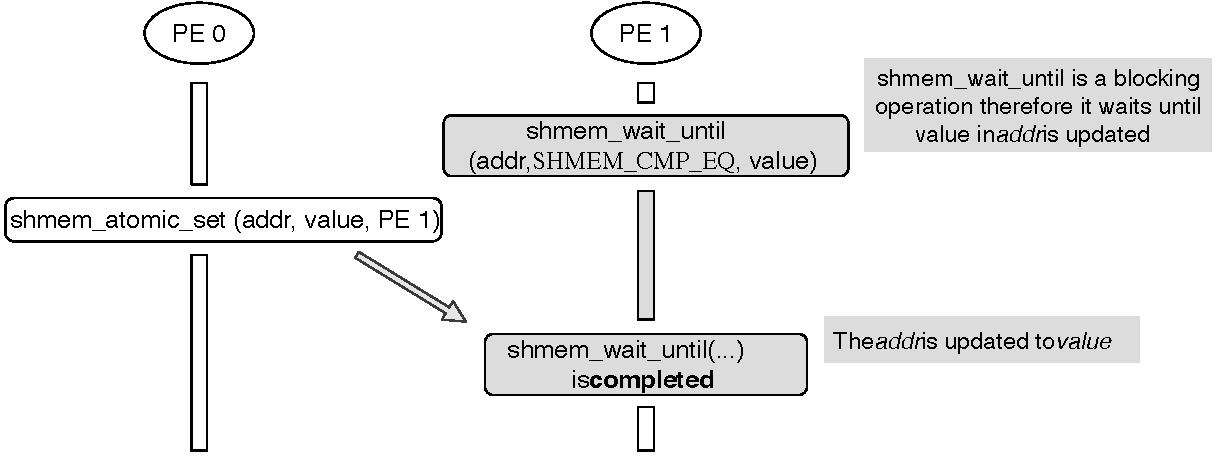
\includegraphics[width=0.7\textwidth]{figures/wait}}
\end{tabular}

\begin{tabular}{p{0.2\textwidth} | p{0.7\textwidth}}
{}
&
Waits for a symmetric variable to be updated by a remote \ac{PE}. Should be
used when computation on the local \ac{PE} cannot proceed without the value that
the remote \ac{PE} is to update. \tabularnewline
\hline
\end{tabular}

\begin{tabular}{p{0.2\textwidth} | p{0.7\textwidth}}

{Ordering puts issued by a local \ac{PE}} \\
\FUNC{shmem\_fence}
&
\raisebox{-\totalheight}{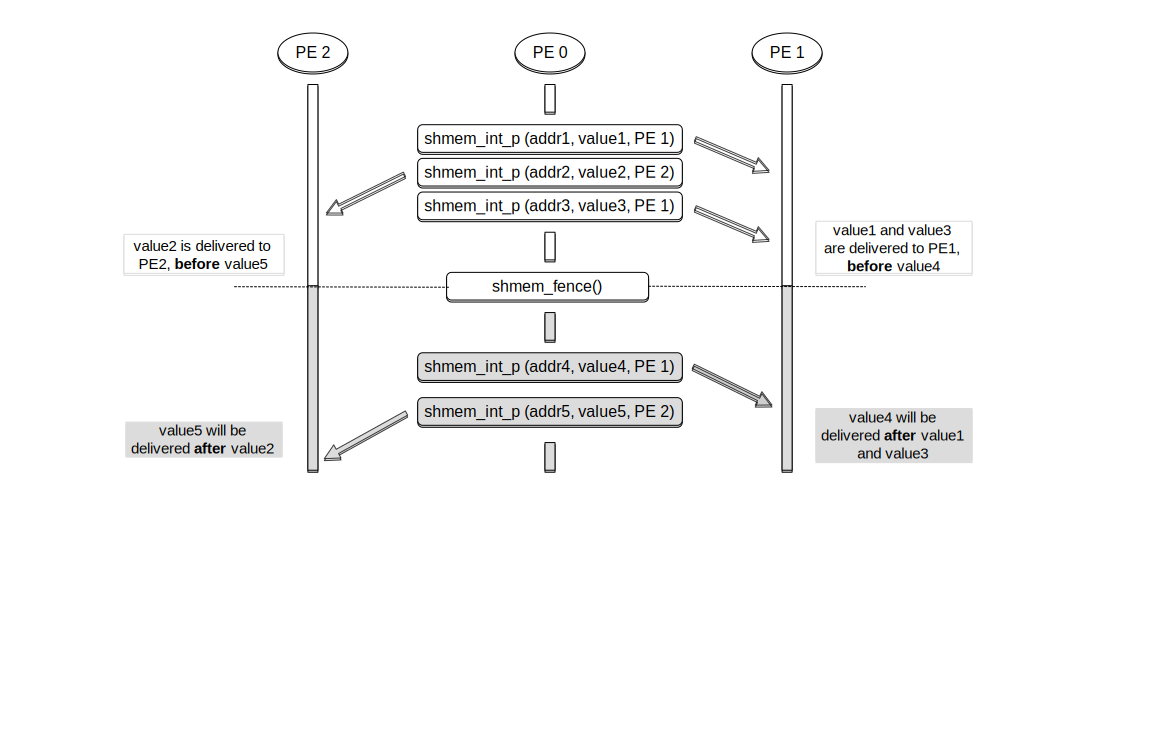
\includegraphics[width=0.7\textwidth]{figures/fence}}
\end{tabular}

\begin{tabular}{p{0.2\textwidth} | p{0.7\textwidth}}
{}
&
All \PUT{}, \ac{AMO}, store, and nonblocking \PUT{} routines on symmetric data issued to
same \ac{PE}  are guaranteed to be delivered  before Puts (to the same \ac{PE})
issued after the \FUNC{fence} call. \tabularnewline
\hline
\end{tabular}

\begin{tabular}{p{0.2\textwidth} | p{0.7\textwidth}}
\hline
\textbf{\openshmem  \ac{API}} & \centering \textbf{Working of \openshmem \ac{API}} \tabularnewline
\hline
\hline
{Ordering puts issued by all \ac{PE} }\\
\FUNC{shmem\_quiet}
&
\raisebox{-\totalheight}{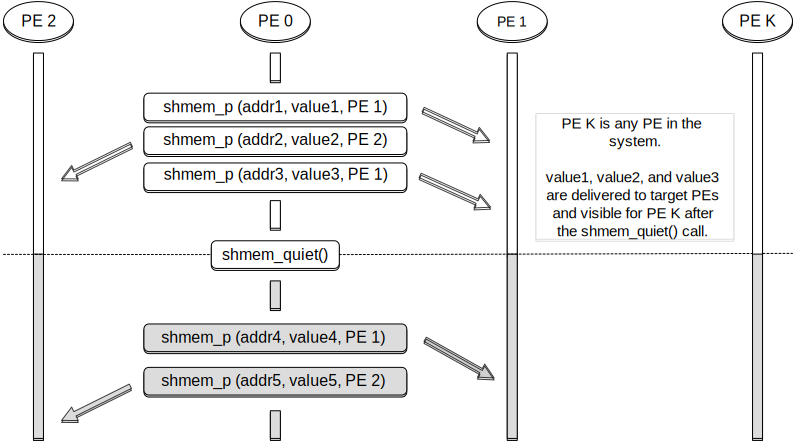
\includegraphics[width=0.7\textwidth]{figures/quiet}}
\end{tabular}

\begin{tabular}{p{0.2\textwidth} | p{0.7\textwidth}}
{}
&
{All \PUT{}, \ac{AMO}, store, and nonblocking \PUT{} and \GET{} routines on symmetric data issued by a
local \ac{PE} to all  remote \acp{PE} are guaranteed to be completed and visible
once quiet returns. This routine should be used when all remote writes issued by
a local \ac{PE} need to be visible  to all other \acp{PE} before the local
\ac{PE} proceeds. } \tabularnewline
\hline
\end{tabular}


\begin{tabular}{p{0.2\textwidth} | p{0.7\textwidth}}
Collective synchronization over an active set \\
\FUNC{shmem\_barrier}
&
\raisebox{-\totalheight}{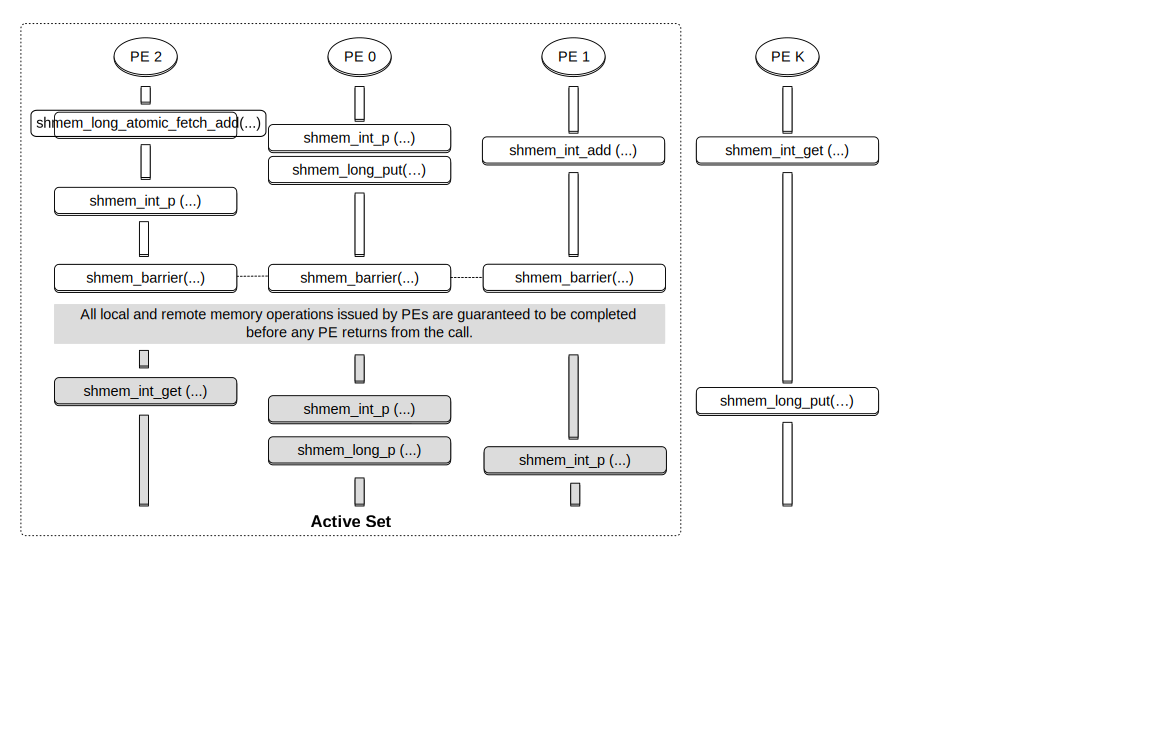
\includegraphics[width=\textwidth]{figures/barrier}}
\end{tabular}

\begin{tabular}{p{0.2\textwidth} | p{0.7\textwidth}}
{}
&
{All local and remote memory operations issued by all \acp{PE} within the
active set are guaranteed to be completed before any \ac{PE} in the
active set returns from the call. Additionally, no \ac{PE} shall return from the
barrier until all \acp{PE} in the active set have entered the same barrier
call. This routine should be used when synchronization as well as completion of
all stores and remote memory updates via \openshmem is required over a sub set
of the executing \acp{PE}.} \tabularnewline
\hline
\end{tabular}

\begin{tabular}{p{0.2\textwidth} | p{0.7\textwidth}}
\hline
\textbf{\openshmem  \ac{API}} & \centering \textbf{Working of \openshmem \ac{API}} \tabularnewline
\hline
\hline
{Collective synchronization over all \acp{PE}} \\
 \FUNC{shmem\_barrier\_all}
&
\raisebox{-\totalheight}{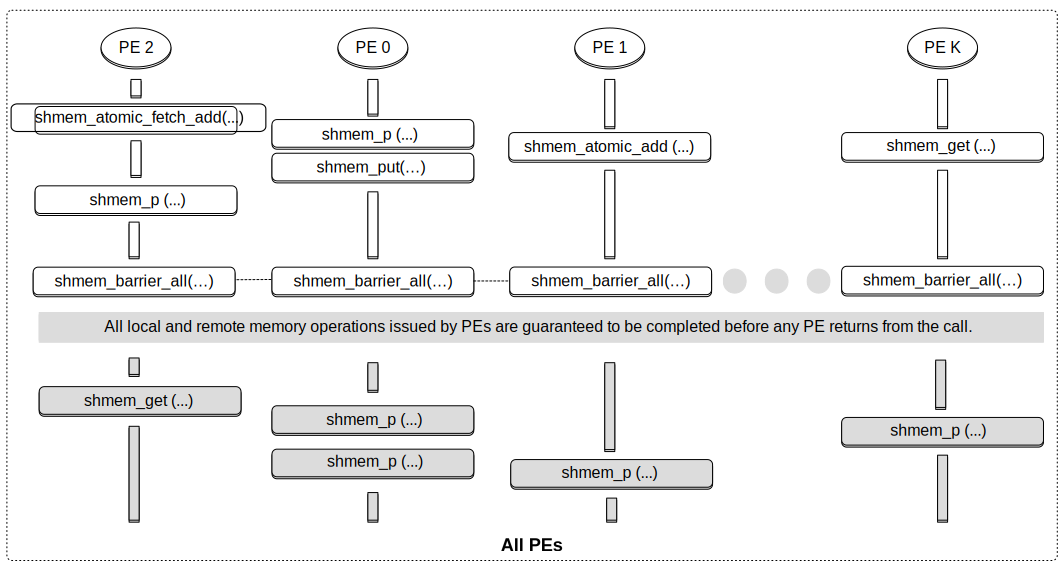
\includegraphics[width=0.8\textwidth]{figures/barrierall}}
\end{tabular}

\begin{tabular}{p{0.2\textwidth} | p{0.7\textwidth}}
{}
&
{All local and remote memory operations issued by all \acp{PE} are guaranteed to
be completed before any \ac{PE} returns from the call. Additionally no \ac{PE}
shall return from the barrier until all \acp{PE} have entered the same
\FUNC{shmem\_barrier\_all} call. This routine should be used when
synchronization as well as completion of all stores and remote memory updates
via \openshmem is required over all \acp{PE}. } \tabularnewline
\hline
\end{tabular}
\clearpage
